\chapter{IoT}
Sempre più spesso si parla di Internet delle cose, o IOT, con questo termine si
intende un evoluzione delle applicazioni legate al settore mobile, al settore
della home automation e al settore embedded.  In questo scenario ogni oggetto il
quale contiene un sensore sarà connesso ad Internet. 
Avvalendosi di questa
connessione , i vari dati raccolti vengono inviati ad un server il quale ha il
compito di analizzarli e renderli disponibili al utente finale.  Avendo la
possibilità di processare il dato nel cloud ogni end devices sarà composto da
una parte  hardware di ridotta complessità riuscendo a mantenere contenuto il
prezzo finale. 
Sebbene il numero di dispositivi "smart" è in rapida crescita, i servizi che
l'IoT offre saranno il vero valore aggiunto. Aziende e enti pubblici stanno
investendo e mettendo a disposizione all'utente finale, sempre più servi in
grado di adattarsi a seconda dei dati provenienti da questi devices.  Gartner
stima  20 miliardi di dispositivi IoT per il 2020, e un investimento annuo pari
a circa 5\$ trilioni di dollari \cite{gartner2016}. 

\begin{table}[h]
        \centering
        \begin{tabular}{l|c|c|c|c}
                Categoria  & 2016 & 2017 & 2018 & 2019 \\
                \hline
                Consumer  & 3963 & 5244,3 & 7063,3 & 12863 \\
                Business  & 1418 & 2135.4 & 4152,7 & 3171  \\
                Totale    & 6381 & 8380   & 11196  & 20415 \\
        \end{tabular}
        \caption{Stima di dispositivi IoT (Milioni di unità) Gartner\cite{gartner2016}}
\end{table}

In contrasto a tutto ciò, la capacità delle aziende di applicare tecniche di
data analytics per far fruttare la grande quantità di dati ricevuti, deve ancora
maturare. Secondo un articolo pubblicato da Verizon, si stima che solo il 92\% delle
aziende usa meno del 25\% dei dati raccolti e che circa il 50\% ha in previsione
di utilizzare più del 25\% di dati nei prossimi due anni \cite{VerizionIoT}

\begin{figure}[h]
        \centering 
                \includegraphics[width=10cm]{iot_devices}
        \caption{Numero di dispositivi per anno}
\end{figure}

Questa rapida crescita ha portato alla ricerca è sviluppo di nuove soluzioni 
tecnologiche per supportare il carico di dispositivi simultaneamente connessi 
alla rete, senza avere un degrado evidente delle performance.
Per non alterare il \emph{QoS} Quality of Service della rete , hardware e
software dovranno essere rivisti insieme alla topologia di rete utilizzata. Alla
base di queste nuove tipologie di rete troviamo :

\begin{itemize}
\item \textbf{Scalabilità}: Dato l'elevato numero di devices previsti nei scenari
urbani ed industriali, la network technology alla base della rete dovrà essere 
adattabile, in modo dinamico, al carico di dispositivi connessi.
\item \textbf{Costo unitario}: Il costo del end device, dovrà essere conveniente
per garantire la più ampia fetta di mercato.
\item \textbf{Durata della batteria}: La maggior parte dei dispositivi sarà
alimentata tramite batteria. Inoltre la maggior parte dei dispositivi verranno
utilizzati in applicazioni nelle quali è prevista una durata minima della
batteria di circa una decina d'anni. 
\item \textbf{Costo computazionale}: La modulazione alla base di queste nuove
tipologie di rete, dovrà essere concepita in modo da non avere un costo
computazionale elevato in modo tale da contenere il costo dell'hardware .
\item \textbf{Distanza}: La necessità di utilizzare questi devices in ambienti
difficili o rurali, rende necessario il poter instaurare comunicazioni a
chilometri di distanza.\improvement{riscrivere}
\item \textbf{Sicurezza}: Lo scambio dei dati dovrà avvenire in maniera sicura,
implementando lo scambio di diti in forma criptata.
\item \textbf{Tolleranza ai guasti}: Il mal  funzionamento di un nodo  non dovrà
compromettere il funzionamento dell'intera rete  a lui connessa. 
\end{itemize}

\begin{figure}[h]
\centering 
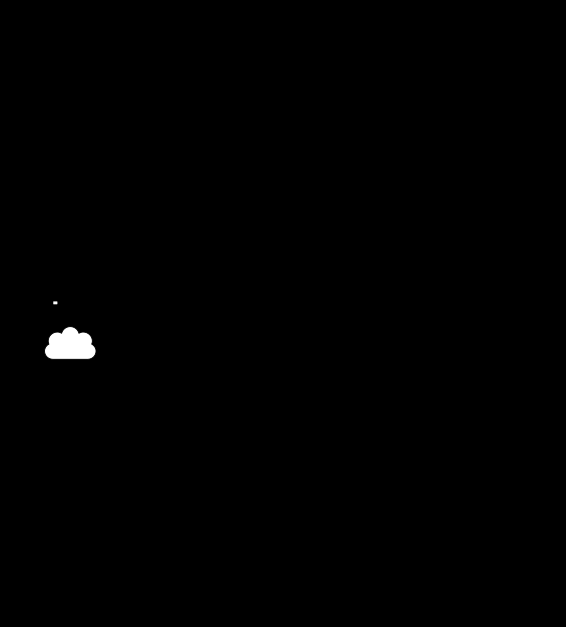
\includegraphics[width=10cm]{three-layer}
\caption{Layer del IoT}
\end{figure}

Vari tipi di architetture di rete sono stati proposti per realizzare questa
nuova infrastruttura. Per quanto le varie proposte si basano su tecnologie
differenti, è possibile individuare tre layer comuni 
\begin{itemize}
\item \textbf{Device layer} formato da tutti i dispositivi che collezionano dati
e sono connessi alla rete.
\item \textbf{Network layer} La struttura della rete, la quale permette di
connettere i vari devices in modo che possano scambiare i dati tra di loro o
inviarli ad un data-center.
\item \textbf{Application layer} il quale interpreta e utilizza i dati ricevuti.
\end{itemize}

Attualmente sono diversi i concorrenti che provano ad affermarsi nel settore
del IoT proponendo soluzioni diverse. Nei seguenti capitoli ci sarà un analisi
generale delle varie topologie proposte, in particolare verrà analizzata la
tecnologia Lora ed il protocolla LoraWAN.

